\begin{frame}
	\frametitle{The CarpentriesOffline Solution}
	\framesubtitle{Making it easier for non-specialists}
		
	\begin{columns}[c]
		\begin{column}{.65\linewidth}
			\begin{itemize}
				\item Downloadable image for booting RPi​
				\item No specialised HPC knowledge required to set up
				\item Community maintained (The Carpentries way)
				\item HPC Lesson material adapted for miniHPC
				\item Expandable with regards to hardware and software
				\item Also suitable for HPC hardware and config training
			\end{itemize}
		\end{column}
		
		\begin{column}[c]{.35\linewidth}
			\begin{figure}
				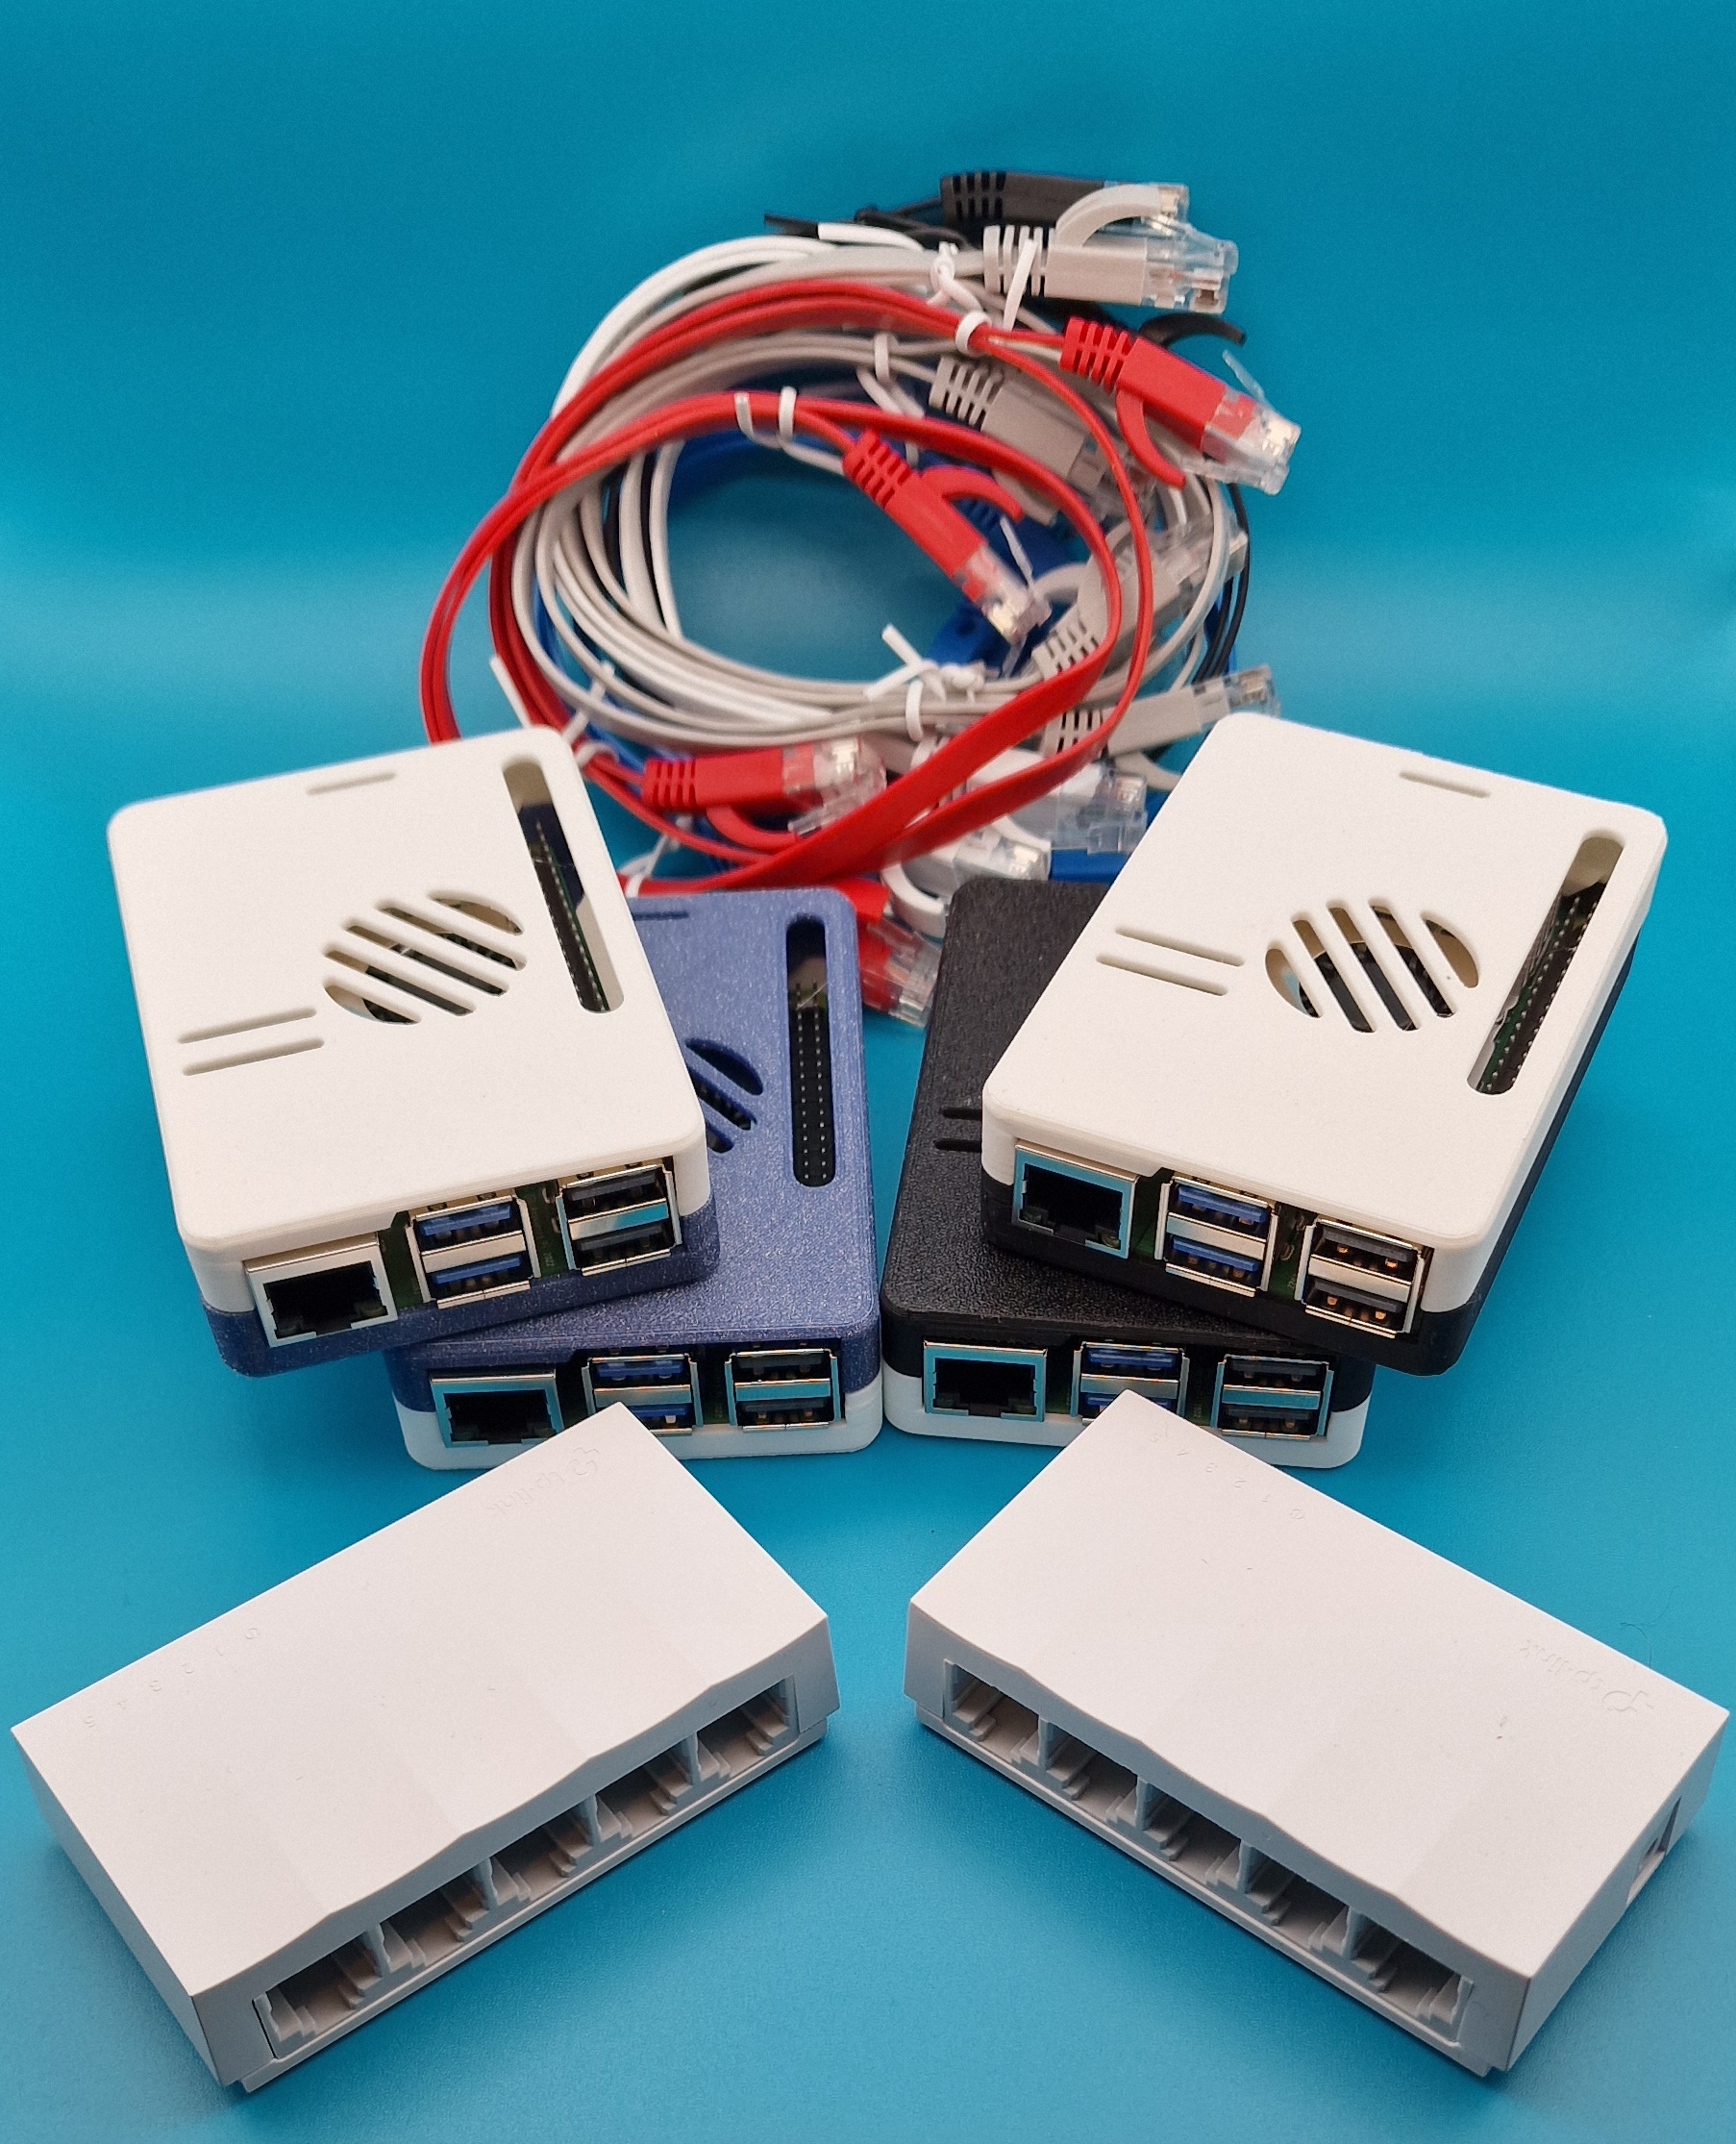
\includegraphics[width=.8\textwidth]{images/training_kit.png}
			\end{figure}
		\end{column}
	\end{columns}
 \end{frame}